\documentclass[tikz]{standalone}
\usepackage{pgfplots}
\pgfplotsset{compat=1.18} % Use a recent compat version
\begin{document}
	
	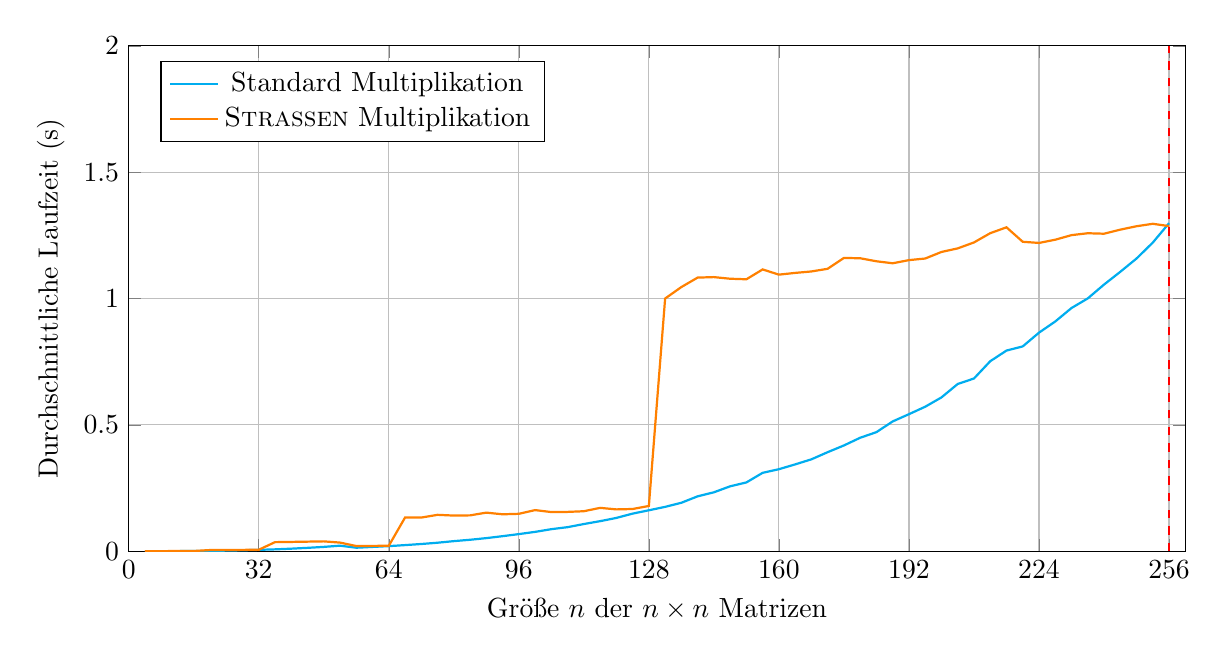
\begin{tikzpicture}
		\begin{axis}[	
			width=15cm, % Setzt die Breite der Grafik
			height=8cm, % Optional: Setzt die Höhe der Grafik
			xlabel={Größe $n$ der $n \times n$ Matrizen},
			ylabel={Durchschnittliche Laufzeit (s)},
			xmin=0, xmax=260,
			ymin=0, ymax=2,
			xtick={0,32,...,256},
			ytick={0,0.5,...,2},
			legend pos=north west,
			grid=major
			]
			\addplot[color=cyan, thick] table {
				4   0.000027
				8   0.000101
				12  0.000312
				16  0.000708
				20  0.001350
				24  0.002304
				28  0.003644
				32  0.005369
				36  0.007291
				40  0.010007
				44  0.013256
				48  0.017039
				52  0.021834
				56  0.013749
				60  0.016938
				64  0.020041
				68  0.024157
				72  0.028486
				76  0.033549
				80  0.039826
				84  0.045262
				88  0.051738
				92  0.059471
				96  0.067689
				100 0.076471
				104 0.087148
				108 0.095150
				112 0.107501
				116 0.118892
				120 0.131730
				124 0.148736
				128 0.161912
				132 0.175445
				136 0.191708
				140 0.217163
				144 0.233093
				148 0.256793
				152 0.272154
				156 0.310149
				160 0.324504
				164 0.343517
				168 0.363632
				172 0.391884
				176 0.418512
				180 0.448960
				184 0.471133
				188 0.513541
				192 0.542235
				196 0.571728
				200 0.608602
				204 0.661712
				208 0.683460
				212 0.751752
				216 0.793948
				220 0.810436
				224 0.864762
				228 0.909023
				232 0.962290
				236 1.000335
				240 1.055068
				244 1.105579
				248 1.158183
				252 1.221187
				256 1.298067
			};
			\addlegendentry{Standard Multiplikation}
			
			\addplot[color=orange, thick] table {
				4   0.000045
				8   0.000142
				12  0.000698
				16  0.000808
				20  0.004538
				24  0.004827
				28  0.005236
				32  0.005674
				36  0.035827
				40  0.036722
				44  0.037815
				48  0.038888
				52  0.034057
				56  0.020460
				60  0.020990
				64  0.021484
				68  0.133145
				72  0.133083
				76  0.143920
				80  0.141013
				84  0.141792
				88  0.152629
				92  0.146050
				96  0.147936
				100 0.162647
				104 0.154874
				108 0.155554
				112 0.158186
				116 0.171497
				120 0.165475
				124 0.166968
				128 0.179074
				132 0.999888
				136 1.045382
				140 1.082742
				144 1.084697
				148 1.078266
				152 1.076065
				156 1.115063
				160 1.094453
				164 1.101307
				168 1.107035
				172 1.117648
				176 1.160525
				180 1.159266
				184 1.147314
				188 1.139447
				192 1.151873
				196 1.158231
				200 1.184203
				204 1.198355
				208 1.221877
				212 1.258453
				216 1.281702
				220 1.224457
				224 1.219905
				228 1.232622
				232 1.250792
				236 1.258274
				240 1.256394
				244 1.272495
				248 1.285980
				252 1.295652
				256 1.286444
			};
			\addlegendentry{\textsc{Strassen} Multiplikation}
			
			% Vertical dashed line at n = 256
			\addplot[red, thick, dashed] coordinates {(256, 0) (256, 2)};
		\end{axis}
	\end{tikzpicture}
\end{document}